\chapter{Design}

    \paragraph*{}
        A significant amount of time was spent on the design of the system.
        A careful consideration was given to working of the frontend and the backend. The system was designed to be as modular as possible.
        The system was designed to be able to be used in multiple ways.
        Special attention to the design of the frontend was given including contrast ratios, colors and rhythm was given. User experience was also given a high priority. 



    \section{Design Patterns}
        \begin{itemize}
            \item{State}

            The useState hook in react exposes a way to change the state of the component, this allows us to re-render the ui whenever change the state of the component. The functional component might behave differently depending on the state of the component. This is how a the state pattern is used here.
            
            \begin{figure}[h]
                \centering
                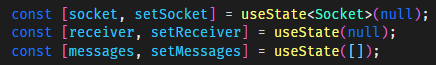
\includegraphics[width=0.8\textwidth]{images/useState.png}
                \caption{State Pattern}
                \label{fig:state}
            \end{figure}

            \pagebreak

            \item{Memento}
            
            The useMemo hook allows us to memoize the output of the component. This is how the memento pattern is used here. Here we are memoizing the slotList. This is done to avoid re-calculating and re-sorting the slotList when the component re-renders.

            \begin{figure}[h]
                \centering
                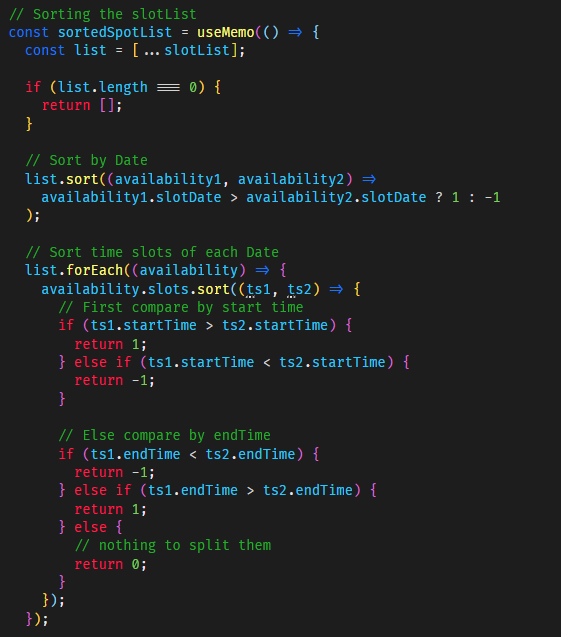
\includegraphics[width=0.8\textwidth]{images/useMemo.png}
                \caption{Memento Pattern}
                \label{fig:memento}
            \end{figure}
            
        \end{itemize}

        \pagebreak

        \section{Frontend}
           \subsection{Wireframe}
                \paragraph*{}
                    Before the development of the UI the design of the wireframe was considered. A wireframe of the UI was created that gave the general understanding of how the UI will be broken into components.

                    \begin{figure}[h]
                        \centering
                        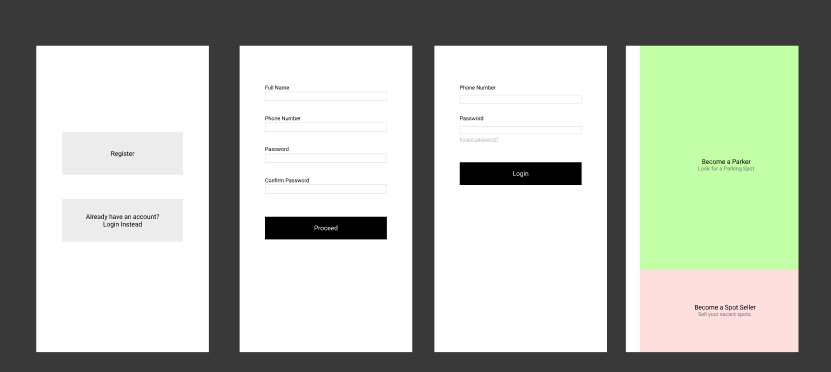
\includegraphics[width=0.6\textwidth]{images/homepageWireframe.png}
                        \caption{Homepage Wireframe}
                        \label{fig:homepageWireframe}
                    \end{figure}
 
                    \begin{figure}[h]
                        \centering
                        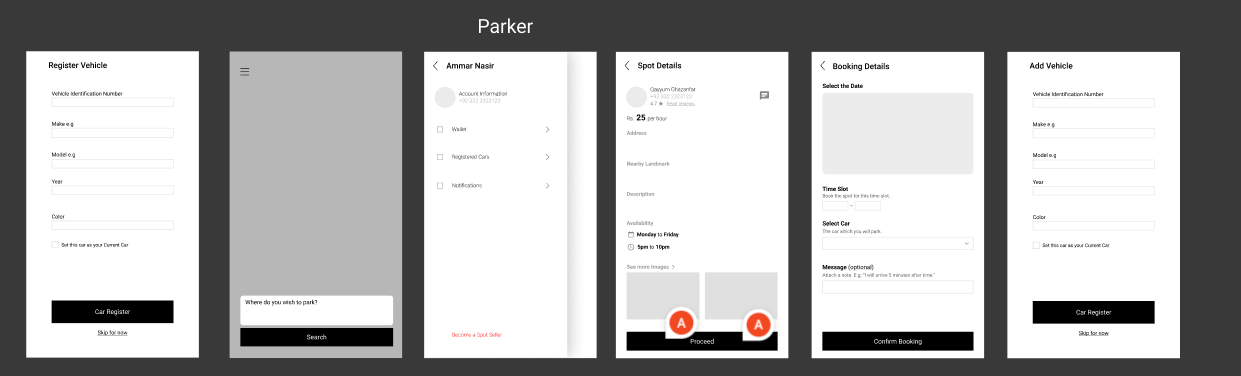
\includegraphics[width=0.6\textwidth]{images/parkerWireframe.png}
                        \caption{Parker Wireframe}
                        \label{fig:parkerWireframe}
                    \end{figure}

                    \begin{figure}[h]
                        \centering
                        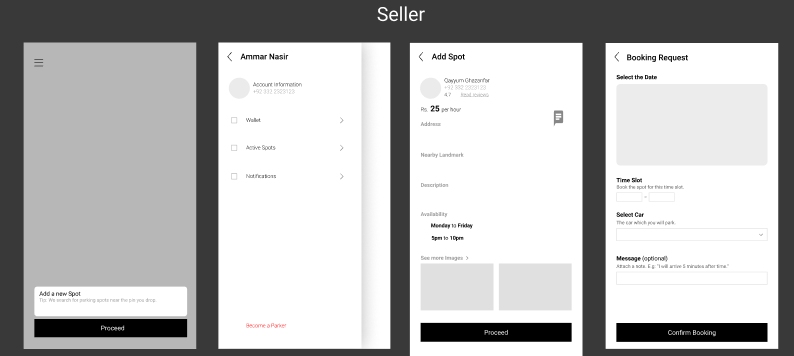
\includegraphics[width=0.6\textwidth]{images/sellerWireframe.png}
                        \caption{Seller Wireframe}
                        \label{fig:sellerWireframe}
                    \end{figure}


                \subsection{UI}
                \paragraph*{}
                    At the start of UI design the Font, Colors and Design schemes were solidified to ease the process and keep the consistency throughout the application. The aim was to make the UI look and feel like one cohesive application.

                    \begin{figure}[h]
                        \centering
                        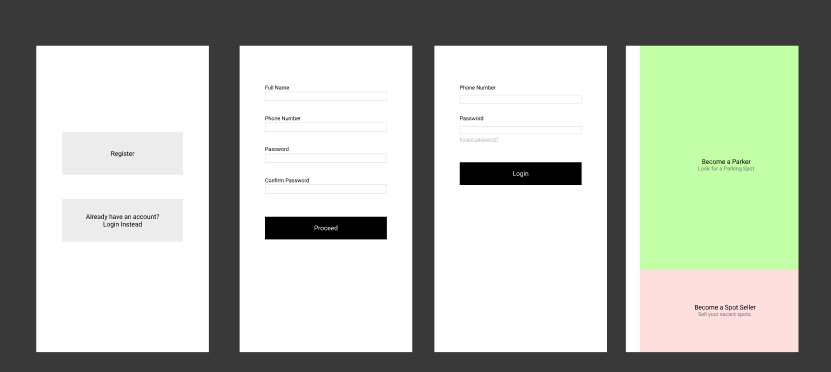
\includegraphics[width=0.6\textwidth]{images/homepageWireframe.png}
                        \caption{Homepage Wireframe}
                        \label{fig:homepageWireframe}
                    \end{figure}
    
                    \begin{figure}[h]
                        \centering
                        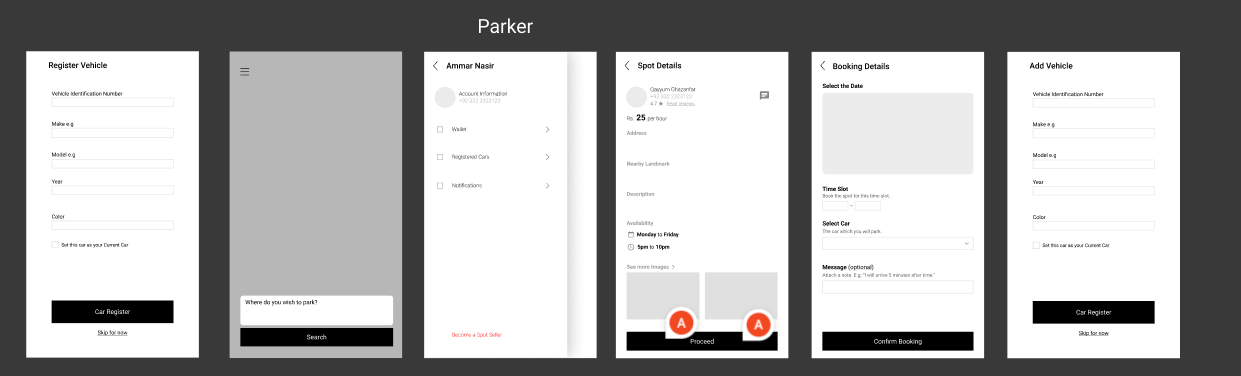
\includegraphics[width=0.6\textwidth]{images/parkerWireframe.png}
                        \caption{Parker Wireframe}
                        \label{fig:parkerWireframe}
                    \end{figure}

                    \begin{figure}[h]
                        \centering
                        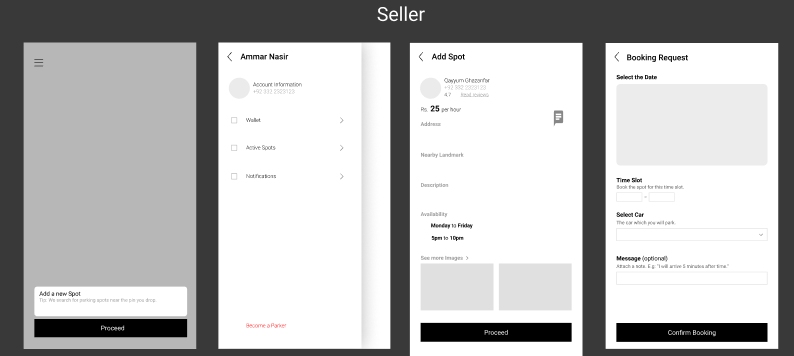
\includegraphics[width=0.6\textwidth]{images/sellerWireframe.png}
                        \caption{Seller Wireframe}
                        \label{fig:sellerWireframe}
                    \end{figure}

